\section{Controller Setup}
\label{chap:Controller}
% Talk about definition and setup of the controller in MATLAB, describing all the parameters set, then talk about the simulink model and then talk about the ``partitioning" of functionalities for the tests (Path following - Static avoidance- Dynamic avoidance)
% In this section we will describe in detail how we implemented the controller in the MATLAB/Simulink environment.
% 1) Implementazione  MPC in Matlab
% 2) Implementazione MPC in Simulink
% 3) Partitioning delle funzionalità del MPC

% 1) Together Copy and paste from misc.tex MATLAB implementation


Matlab's Model Predictive Control Toolbox provides functions, an app, and Simulink blocks for designing and simulating controllers using linear and nonlinear model predictive control (MPC) \cite{MPCToolbox}. Thanks to the toolbox we specified the plant model, horizons, constraints, and weights. By running closed-loop simulations, we evaluated controller performance and adjusted its behavior by varying weights and constraints at run time.

\subsection{MPC Initialisation}
Initialisation phase requires the definition of all the parameters needed for the execution of the controller.
First of all we have created a MPC object passing as input the discretized state-space model of the plant, the prediction horizon and the control horizon.
\\Assuming that the car is already traveling at a speed \textit{V}, the initial conditions for the other states is set taking the first point in the reference path, and for the two inputs it is set equal to zero. Exploiting the function \textit{odometer} we computed the total distance covered by the car following the scenario in order to let the simulation terminates exactly when the road ends.
\\Subsequently we defined the constraints on inputs (Table \ref{tab:steering} and \ref{tab:throttle}), constraints on the state and the weights for the cost function, which correctly tuned, guarantee that the vehicle follows the reference without going off the road.
The cost function of the MPC takes as input the weights for all the states of the model, the input manipulated variables and the manipulated variables rate. In our case, the states of the plant model are four, and to tune the controller, we have to give a weight to each one of them. Our choice is to give the same weight to states \textit{x} and \textit{y}, which represent the position of the vehicle in the reference frame, and then to play with the weights on angle $\theta$ and \textit{v} to tune the MPC.\\
Moreover we decided to give 0 weight to the manipulated variables.\\
Constant constraints, as the ones defined for the inputs, can be given to the controller directly in the initialisation phase, while constraints on the states, which are time varying, can be passed at runtime my means of the matrices \textit{E}, \textit{F} and \textit{G}. \\
MPC algorithm try to solve the equation:
\begin{equation}
    E \cdot u(k+j) + F \cdot y(k+j)\leq G
    \label{ConstraintEquation}
\end{equation}
for all the steps in the prediction horizon, scanned by index \textit{j}, where \textit{y} is the vector of measured and unmeasured outputs and \textit{u} is the vector of manipulated variables at instant \textit{k}.
% i.e. stays within the lane width limits and is capable to avoid an obstacle when is inside the sensors detection range.





% 2) Alessandro  SIMULINK
\subsection{Simulink Model}

Once the controller has been initialised, all is set to begin the simulation.
In order to run closed-loop simulations a Simulink model has been designed because of the availability of many useful tools to test and validate the model. For the sake of clarity in reading and debugging the whole system, some of the Simulink blocks have been grouped in subsystems and a mask has been applied to some of them. 
In Figure \ref{fig:simulink_main} the main system is depicted: the process simulated by these blocks is coherent with the MPC algorithm described in the previous subsection and the numbers in green enumerate the four major subsystems which will be analyzed below.

\begin{figure}[H]
    \centering
    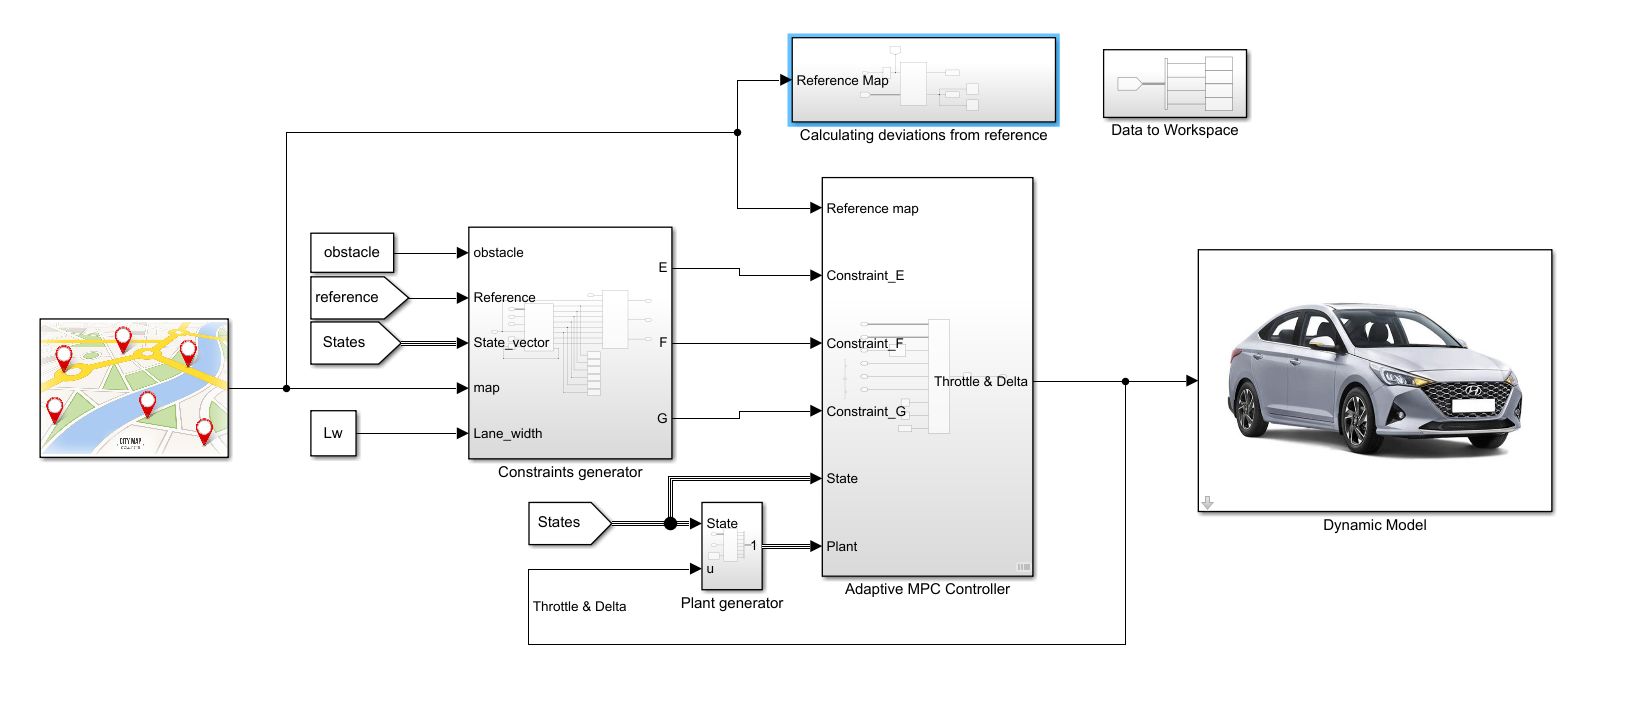
\includegraphics[width=\textwidth]{Figures/simulink_main.png}
    \caption{Simulink main}
    \label{fig:simulink_main}
\end{figure}

 The blocks composing the subsystem \textit{MPC Controller} - subsystem 1 - are showed in Fig.\ref{fig:simulink_mpc}: a block to call the function \textit{LaneKeepConstraint} and the block \textit{Adaptive MPC Controller}. The latter is itself a subsystem containing the matlab block \textit{Adaptive MPC}; beside the reference input \textbf{ref}, there are others eight entry ports used in the adaptive controller block:
 \begin{itemize}
     \item \textbf{model}: updated plant model and nominal operating point. At the beginning of each control interval, this signal modifies the controller object.
     \item \textbf{mo}: Measured outputs. The MPC block uses the measured plant outputs to improve its state estimates.
     \item \textbf{E}: Manipulated variable constraint matrix. The F input port along with the E, G ports specify run-time mixed input/output constraints.
     \item \textbf{F}: Controlled output constraint matrix.
     \item \textbf{G}: Custom constraint vector.
     \item \textbf{y.wt}: Output variable tuning weights. These tuning weights penalize deviations from output references.
     \item \textbf{u.wt}: Manipulated variable tuning weights.  These tuning weights penalize deviations from MV targets.
     \item \textbf{du.wt}: Manipulated variable rate tuning weights. These tuning weights penalize large changes in control moves.
 \end{itemize}     
\begin{figure}[H]
    \centering
    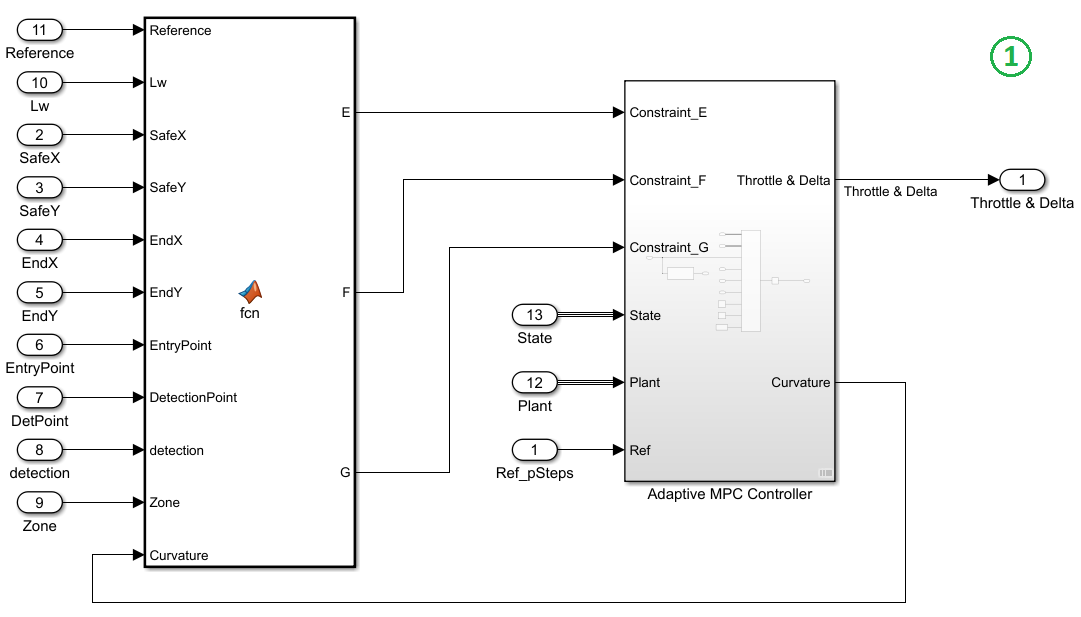
\includegraphics[width=0.9\textwidth]{Figures/simulink_mpc.png}
    \caption{Simulink subsystem: Adaptive MPC controller}
    \label{fig:simulink_mpc}
\end{figure}


The content of the subsystem numbered 2 (see Fig.\ref{fig:simulink_main}) instead, it's displayed in Figure \ref{fig:simulink_deviation}: the main purpose of these blocks is to calculate a deviation from the reference in order to test the controller and will be analyzed in details in the Section \ref{chap:path_following}; in order to pass the proper number of reference way-points, a sampling subsystem is used as a input to the MATLAB function block.
\begin{figure}[H]
    \centering
    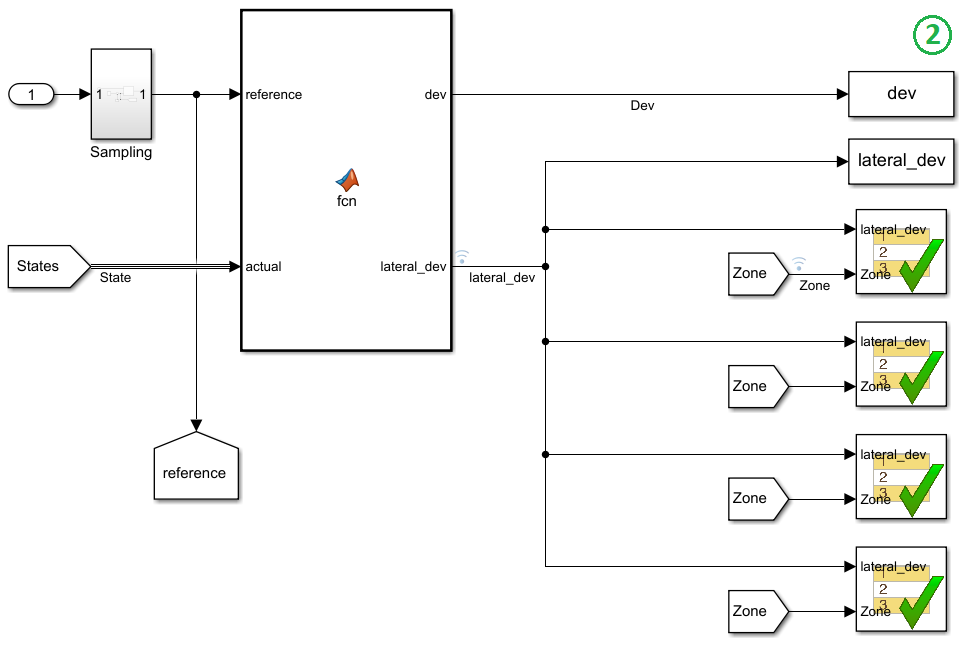
\includegraphics[width=0.9\textwidth]{Figures/simulink_deviation.png}
    \caption{Simulink subsystem to calculate deviations}
    \label{fig:simulink_deviation}
\end{figure}
 
The subsystem \textit{Dynamic Model} displayed in Fig.\ref{fig:simulink_main} has as a mask the picture of an Hyundai Azera, the vehicle whose parameters are used in the simulation. Also for these blocks $-$ Fig.\ref{fig:simulink_dyn_mod}, the main purpose is calling an already designed MATLAB function that in this case is the \textit{VehicleModelCT\_DYN} one, previously described in Section \ref{chap:Vehicle_model}.
\begin{figure}[H]
    \centering
    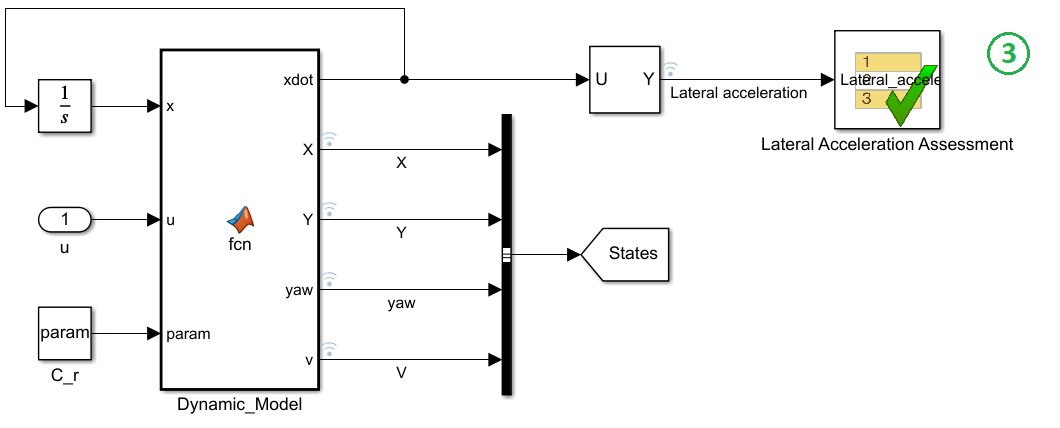
\includegraphics[width=0.9\textwidth]{Figures/simulink_dyn_mod.png}
    \caption{Simulink subsystem: Dynamic Model}
    \label{fig:simulink_dyn_mod}
\end{figure} 

Between the blocks of major interest, the last one described is the \textit{Obstacle detector}, whose content is depicted in Figure \ref{fig:simulink_obstacles}. Again, the main purpose of this subsystem is using the simulink block to call a function. In this case, the \textit{detectionFun} is used to be able to detect multiple obstacles on the road and calculate their relative safe zones.

\begin{figure}[H]
    \centering
    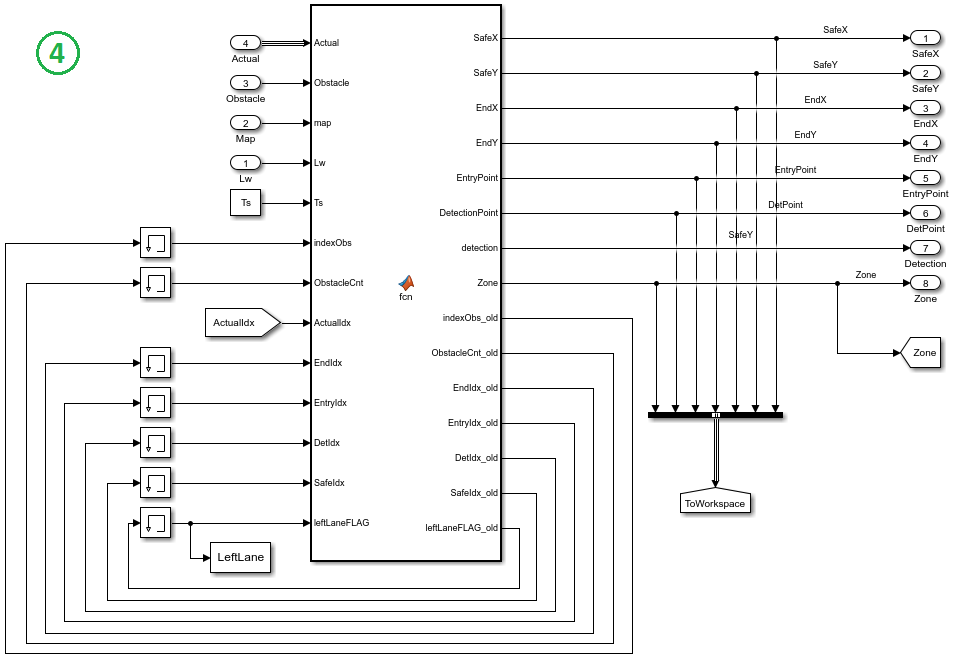
\includegraphics[width=\textwidth]{Figures/simulink_obstacles.png}
    \caption{Simulink obstacles}
    \label{fig:simulink_obstacles}
\end{figure} 



% 3) Gianvincenzo   Partitioning of functionalities
\subsection{Partitioning of the MPC functionalities}
The developed MPC controller is supposed to carry out three main tasks: 
\begin{itemize}
    \item \textbf{Path following}: the car must be able to follow a given reference path without exceeding a predetermined threshold distance;
    \item \textbf{Static obstacle avoidance}: the car must sense and dodge any kind of stationary obstacle present on the road i.e. road construction sites, holes, trees,  car accident, etc.;
    \item \textbf{Dynamic obstacle avoidance}: the car has the ability to perform overtaking maneuvers in the event that other moving vehicles, cyclists, pedestrians or animals are present in the same lane. The avoidance maneuver must be accomplished whether they are traveling in the same direction as the vehicle or in the opposite one.
\end{itemize}
Figure \ref{fig:dynamic_avoidance} shows how the ego-car (red) performs the overtaking maneuver: firstly it analyze the surrounding thanks to the on-board sensors and if it has enough space to achieve the lane change accordingly to the position and speed of the two moving obstacle (white cars) it plans the trajectory to follow to achieve the avoidance (blue path). Once the ego-car has planned a feasible path it starts to steer and accelerate arriving to the middle lane overtaking the car in the rightmost lane.

\begin{figure}[H]
    \centering
    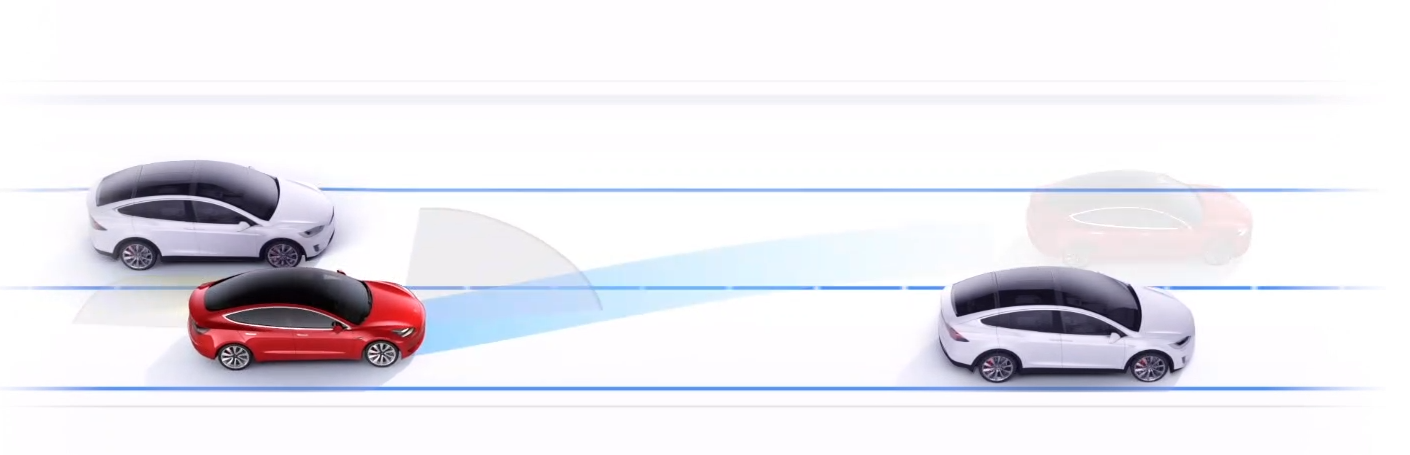
\includegraphics[width=1\textwidth]{Figures/dynamic_avoidance.png}
    \caption{Dynamic obstacle avoidance maneuver on a three lanes road}
      \label{fig:dynamic_avoidance}
\end{figure}
In order to perform the path following task the MPC collects at each timestep the successive waypoints of the map for the duration of the prediction horizon and elaborates an optimal trajectory and control action to minimize the a cost function of the controller.
\\Things get harder when obstacles are present on the road, either they are static or moving: we assumed to know ``a priori" the position of the static obstacle or the trajectory that the moving obstacle is following, in such way thanks to the MATLAB function \textit{``detectionFun"} we augmented the algorithm used for the path following with the capability to detect obstacles within the sensing range of the vehicle, thus allowing to promptly start and execute the avoidance maneuver always being outside the so called \textit{``safe zone"} of the obstacle.\\ Figure \ref{fig:static_avoidance_example} plots an example scenario for static obstacle avoidance, where: 
\begin{itemize}
    \item the \textbf{ego car} is represented by the green dot with the black boundary;
    \item the \textbf{horizontal lanes} are represented by the dashed blue lines;
    \item the \textbf{static obstacle} is represented by the red x with the black boundary;
    \item the \textbf{safe zone} is highlighted by the dashed red boundary.
\end{itemize} 

\begin{figure}[H]
    \centering
    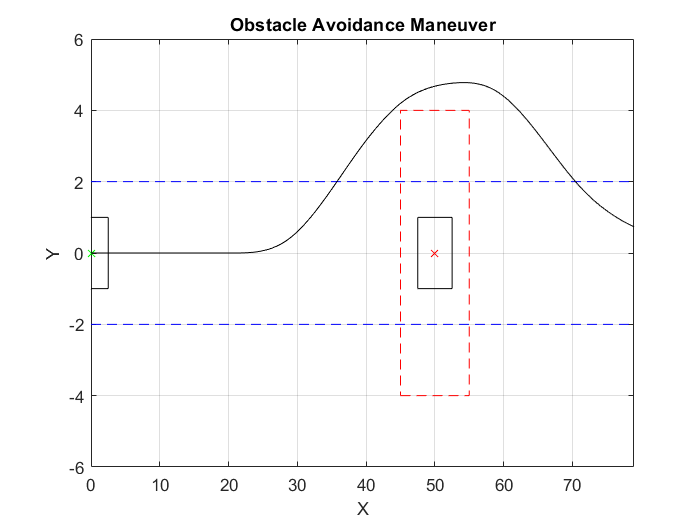
\includegraphics[width=1\textwidth]{Figures/static_avoidance_example.png}
    \caption{Example of static obstacle avoidance maneuver}
      \label{fig:static_avoidance_example}
\end{figure} 
